\documentclass[a4paper]{article}

%%%%%%%% CREATE DOCUMENT STRUCTURE %%%%%%%%
%% Language and font encodings
\usepackage[english]{babel}
\usepackage[utf8x]{inputenc}
\usepackage[T1]{fontenc}
%\usepackage{subfig}

%% Sets page size and margins
\usepackage[a4paper,top=3cm,bottom=2cm,left=2cm,right=2cm,marginparwidth=1.75cm]{geometry}

%% Useful packages
\usepackage{amsmath}
\usepackage{graphicx}
\usepackage[colorinlistoftodos]{todonotes}
\usepackage[colorlinks=true, allcolors=blue]{hyperref}
\usepackage{caption}
\usepackage{subcaption}
\usepackage{sectsty}
\usepackage{apacite}
\usepackage{float}
\usepackage{titling} 
\usepackage{blindtext}
\usepackage[colorinlistoftodos]{todonotes}
\usepackage{xcolor}
\definecolor{darkgreen}{rgb}{0.0, 0.4, 0.0}
\graphicspath{ {images/} }
%%%%%%%% DOCUMENT %%%%%%%%
\begin{document}

%%%% Title Page
\begin{titlepage}

\newcommand{\HRule}{\rule{\linewidth}{0.5mm}} 							% horizontal line and its thickness
\center 
 
% University
\textsc{\LARGE Delft University of Technology}\\[1cm]

% Document info
\textsc{\Large Sensing Technologies and Mathematics}\\[0.2cm]
\textsc{\large GEO1001}\\[1cm] 										% Course Code
\HRule \\[0.8cm]
{ \huge \bfseries Assignment: 01}\\[0.7cm]								% Assignment
\HRule \\[2cm]
\large
\emph{Author:}\\
Pratyush Kumar (5359252)\\[1.5cm]													% Author info
{\large \today}\\[5cm]

\includegraphics[width=0.6\textwidth]{images/TU_delft_logo.jpg}\\[1cm] 	% University logo
\vfill 
\end{titlepage}

%%\begin{abstract}
%%Your abstract.
%%\end{abstract}

%%%% SECTIONS
%% Section 1
\newpage
\section*{A1}
The assignment uses data collected from 5 heat stress sensors \cite{Maiullari2020}  placed in the Netherlands during summer. 

The first part of the assignment requires to print out a table containing the mean, variance and the standard deviation of all the variables for each of the given sensors. The Table 1.concludes the mean variance and standard deviations for all variables. It is interesting to note here that the values for sensor E have some significant amount of deviations from the rest of the sensors specially in the mean of variables of wind direction, wind speed and the crosswind speed. Similarly for the variance in wind speed, crosswind speed and headwind speed.  


{
\small
\begin{table}[htbp]
  \centering
  \caption{Descriptive statistics of variables for all sensors.   }
  \resizebox{\textwidth}{!}{%
    \begin{tabular}{llllllllllllllll}
                             & \multicolumn{5}{c}{MEAN}                                                            & \multicolumn{5}{c}{VAR}                                                             & \multicolumn{5}{c}{STD DEV}                                    \\
                             & \textbf{A} & \textbf{B} & \textbf{C} & \textbf{D} & \multicolumn{1}{l|}{\textbf{E}} & \textbf{A} & \textbf{B} & \textbf{C} & \textbf{D} & \multicolumn{1}{l|}{\textbf{E}} & \textbf{A} & \textbf{B} & \textbf{C} & \textbf{D} & \textbf{E} \\
Direction, True              & 209.4      & 183.4      & 183.6      & 198.3      & 224.0                           & 10108.9    & 9977.2     & 7703.4     & 8133.9     & 9308.3                          & 100.5      & 99.9       & 87.8       & 90.2       & 96.5       \\
Wind Speed                   & 1.3        & 1.2        & 1.4        & 1.6        & 0.6                             & 1.3        & 1.3        & 1.4        & 1.7        & 0.5                             & 1.1        & 1.1        & 1.2        & 1.3        & 0.7        \\
Crosswind Speed              & 1.0        & 0.8        & 1.0        & 1.2        & 0.4                             & 0.9        & 0.9        & 1.0        & 1.5        & 0.3                             & 1.0        & 0.9        & 1.0        & 1.2        & 0.6        \\
Headwind Speed               & 0.2        & -0.1       & -0.3       & -0.3       & 0.2                             & 1.0        & 1.3        & 1.3        & 1.2        & 0.3                             & 1.0        & 1.1        & 1.1        & 1.1        & 0.6        \\
Temperature                  & 18.0       & 18.1       & 17.9       & 18.0       & 18.4                            & 15.9       & 16.6       & 16.1       & 16.1       & 19.0                            & 4.0        & 4.1        & 4.0        & 4.0        & 4.4        \\
Globe Temperature            & 21.5       & 21.8       & 21.6       & 21.4       & 21.2                            & 68.2       & 66.0       & 67.9       & 61.2       & 63.2                            & 8.3        & 8.1        & 8.2        & 7.8        & 8.0        \\
Wind Chill                   & 17.8       & 17.9       & 17.8       & 17.8       & 18.3                            & 16.3       & 17.0       & 16.5       & 16.6       & 19.1                            & 4.0        & 4.1        & 4.1        & 4.1        & 4.4        \\
Relative Humidity            & 78.2       & 77.9       & 78.0       & 77.9       & 76.8                            & 376.0      & 408.6      & 374.6      & 389.9      & 406.5                           & 19.4       & 20.2       & 19.4       & 19.7       & 20.2       \\
Heat Stress Index            & 17.9       & 18.0       & 17.8       & 17.9       & 18.3                            & 15.0       & 15.4       & 15.4       & 15.1       & 18.5                            & 3.9        & 3.9        & 3.9        & 3.9        & 4.3        \\
Dew Point                    & 13.6       & 13.5       & 13.5       & 13.5       & 13.6                            & 9.7        & 9.6        & 10.1       & 10.1       & 9.4                             & 3.1        & 3.1        & 3.2        & 3.2        & 3.1        \\
Psychro Wet Bulb Temperature & 15.3       & 15.3       & 15.2       & 15.3       & 15.4                            & 6.9        & 6.8        & 7.2        & 7.0        & 7.0                             & 2.6        & 2.6        & 2.7        & 2.7        & 2.6        \\
Station Pressure             & 1016.2     & 1016.7     & 1016.7     & 1016.7     & 1016.2                          & 38.5       & 36.8       & 37.7       & 35.0       & 38.9                            & 6.2        & 6.1        & 6.1        & 5.9        & 6.2        \\
Barometric Pressure          & 1016.1     & 1016.6     & 1016.7     & 1016.7     & 1016.1                          & 38.5       & 36.8       & 37.7       & 35.0       & 38.9                            & 6.2        & 6.1        & 6.1        & 5.9        & 6.2        \\
Altitude                     & -26.0      & -30.1      & -30.3      & -30.7      & -26.0                           & 2663.6     & 2545.7     & 2608.5     & 2419.7     & 2692.4                          & 51.6       & 50.5       & 51.1       & 49.2       & 51.9       \\
Density Altitude             & 137.3      & 135.6      & 129.6      & 132.4      & 150.8                           & 26510.0    & 26863.3    & 26986.6    & 26516.1    & 29714.9                         & 162.8      & 163.9      & 164.3      & 162.8      & 172.4      \\
NA Wet Bulb Temperature      & 16.0       & 16.0       & 15.9       & 15.9       & 15.9                            & 10.0       & 9.8        & 10.5       & 10.0       & 9.4                             & 3.2        & 3.1        & 3.2        & 3.2        & 3.1        \\
WBGT                         & 17.3       & 17.3       & 17.2       & 17.2       & 17.2                            & 16.1       & 15.8       & 16.5       & 15.5       & 15.5                            & 4.0        & 4.0        & 4.1        & 3.9        & 3.9        \\
TWL                          & 301.4      & 299.5      & 301.9      & 305.3      & 284.1                           & 814.8      & 790.1      & 766.5      & 616.0      & 1289.9                          & 28.5       & 28.1       & 27.7       & 24.8       & 35.9       \\
Direction, Mag               & 208.9      & 183.2      & 183.1      & 197.8      & 223.9                           & 10105.7    & 9975.4     & 7704.6     & 8135.3     & 9268.0                          & 100.5      & 99.9       & 87.8       & 90.2       & 96.3      
\end{tabular}%
}
\label{tab:addlabel}%
\end{table}%
}


\noindent The figures below show the histograms for the temperatures of sensors A to E, figure 1 showing them as separate subplots while Figure 2.  showing in an aggregated for in a single plot. The choice of bins from rice’s rule of thumb for bin selection stands at  \(2 * \sqrt[3]{N} =2 * 13.52851768\) where N for the given data-set is approximately 2500 which gives the number of bins as 26, so 30 stands as a good approximation. 
\\


\begin{figure}[H]
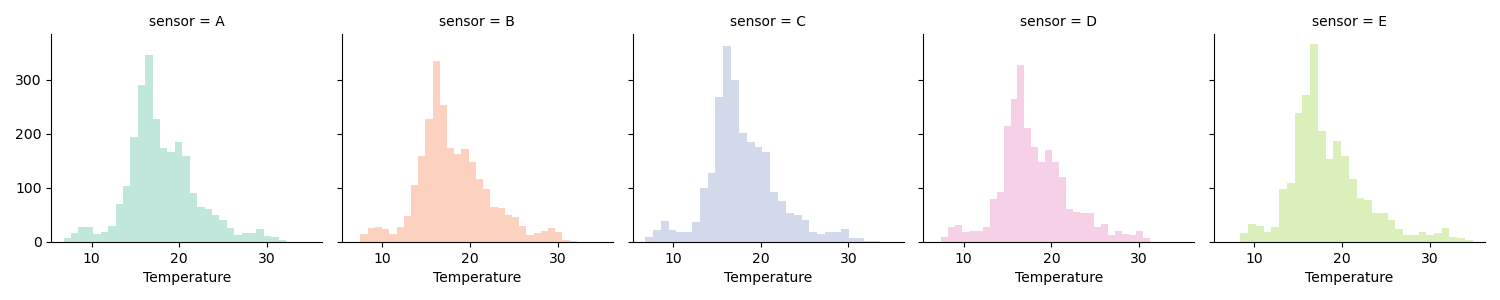
\includegraphics[width=17cm]{images/a1_1.png}
\centering
\caption{Sub-plotted histograms of temperatures variable for sensors A to E, with 30 bins}
\end{figure}


\begin{figure}[H]
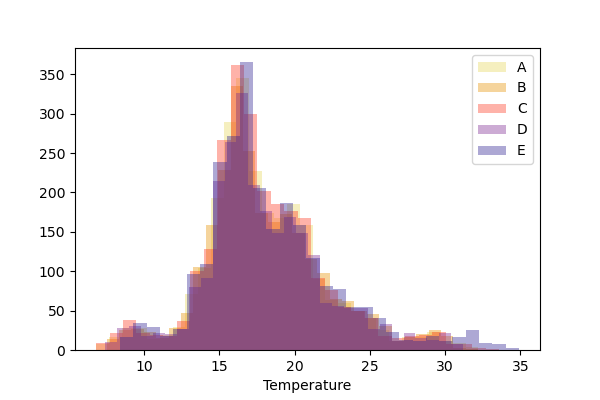
\includegraphics[width=12cm]{images/a1_2.png}
\centering
\caption{Aggregated histograms of temperatures variable for sensors A to E, with 30 bins}
\end{figure}

 When the histograms are plotted with bin sizes of 5 and 50, significant difference in the distribution of the dataset is observed. In the Figure 3. below, It is evident that the distribution has 2 local maximas in the plot with number of bins set as 50 while for the plot where the number of bins are mere 5, the distribution is not so elucidated, and shows a single mode.

\begin{figure}[H]
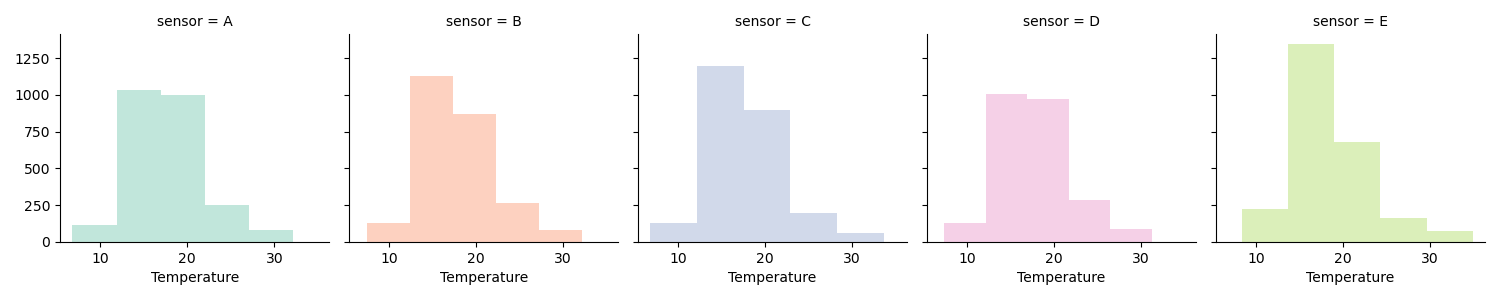
\includegraphics[width=17cm]{images/a1_3.png}
\centering

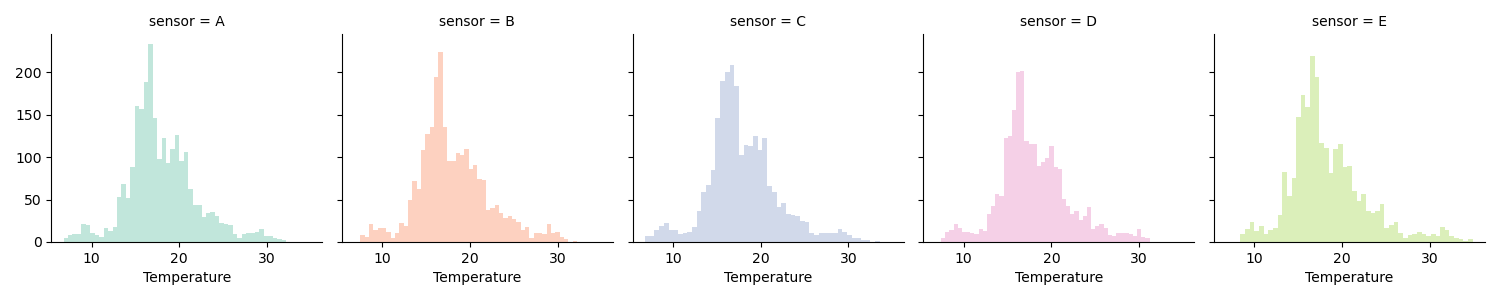
\includegraphics[width=17cm]{images/a1_4.png}
\centering
\caption{Sub-plotted histograms of Temperatures variable for sensors A to E, with 5bins (above) and 50 bins(below)}
\end{figure}

The frequency polygons when plotted and aggregated into a single graph for the sensors look like Figure 4. below. In the plot it is evident that the values from sensor E has a different characteristic than the rest of the sensors when looking at the tail of the plot.

\begin{figure}[H]
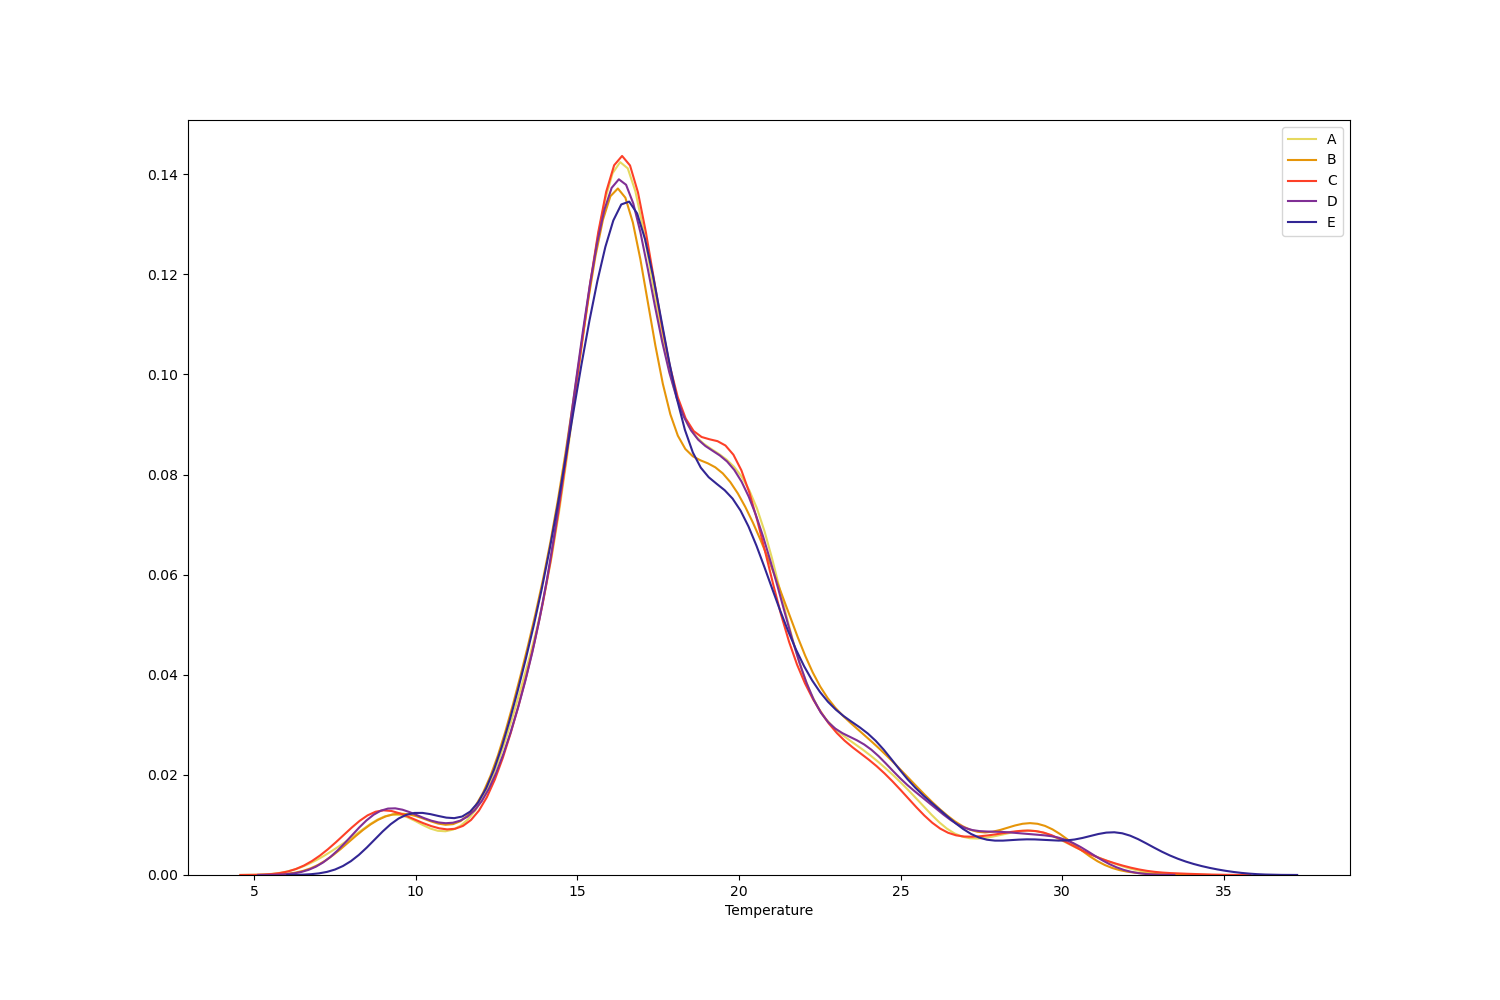
\includegraphics[width=17cm]{images/a1_5.png}
\centering
\caption{Aggregated Frequency Polygons Sensor temperature values }
\end{figure}

The boxplots for sensors A-E for the variables of wind direction , wind speed and temperature. The Wind speed and wind direction box plots for sensor E, both show that there is some variation in the data captured from sensor E.
\begin{figure}[H]
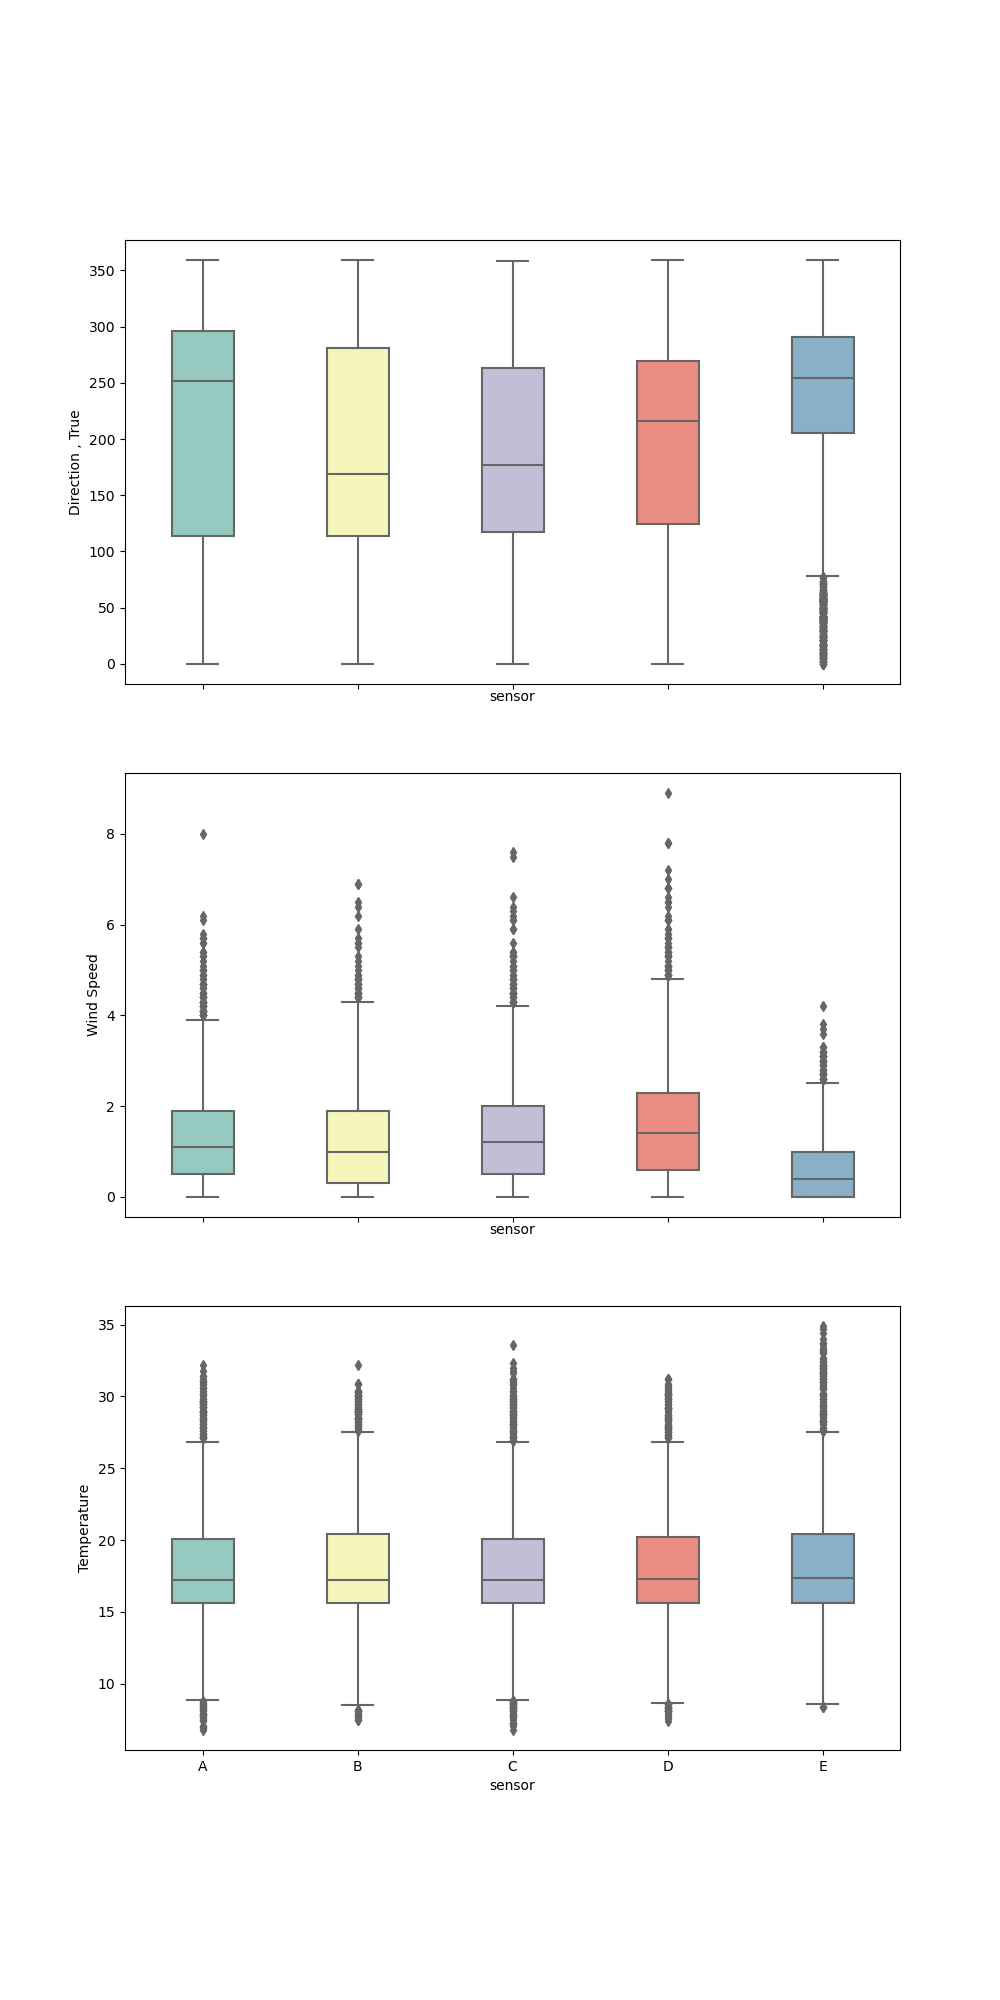
\includegraphics[width=12cm]{images/a1_6.png}
\centering
\caption{Box plots of  Wind Direction, Wind Speed and Temperature values for sensors A to E}
\end{figure}

\newpage
\section{A2}
Below in Figure 6., the PMF, PDF and the CDF of the temperatures values of sensors A,B,C,D,E have been plotted. When compared across all sensors, there seems to be two local maximas in the distribution, with probabilities peaking twice in the range from 15 degree Celsius to 20 degree Celsius. The dataset shows a right skew indicating that the mean is shifted to the right in comparision to the median which is evident from the PMF and the PDF. Comparing the CDF with the PMF and PDF it is visible that 50 \%\ of the dataset lies in the 15-17 degrees range.

\begin{figure}[H]
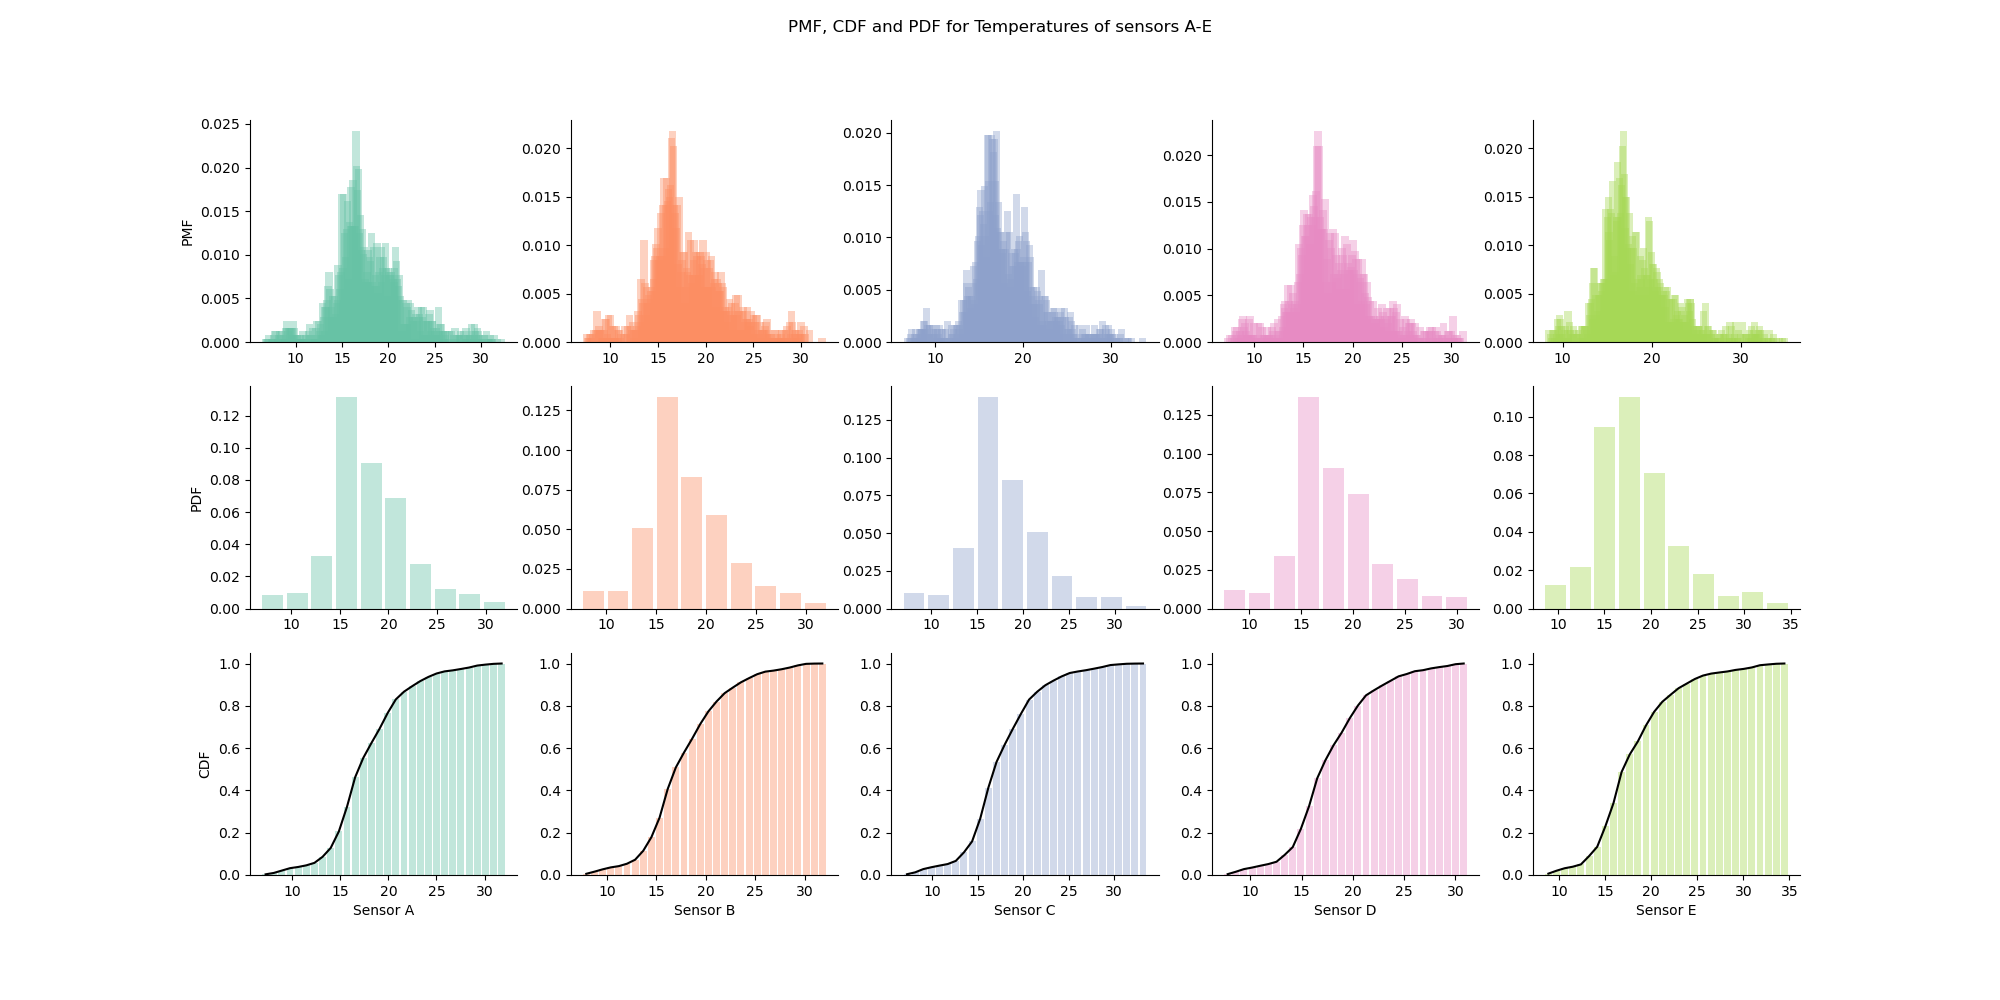
\includegraphics[width=17cm]{images/a2_1.png}
\centering
\caption{PMF, PDF and CDF of temperature values}
\end{figure}

On plotting the Kernel Density Estimate of the wind speeds for all sensors individually along with their Probability density function in Figure 7, it is again visible that sensor E has a different distribution as compared to the remaining sensors. 
\begin{figure}[H]
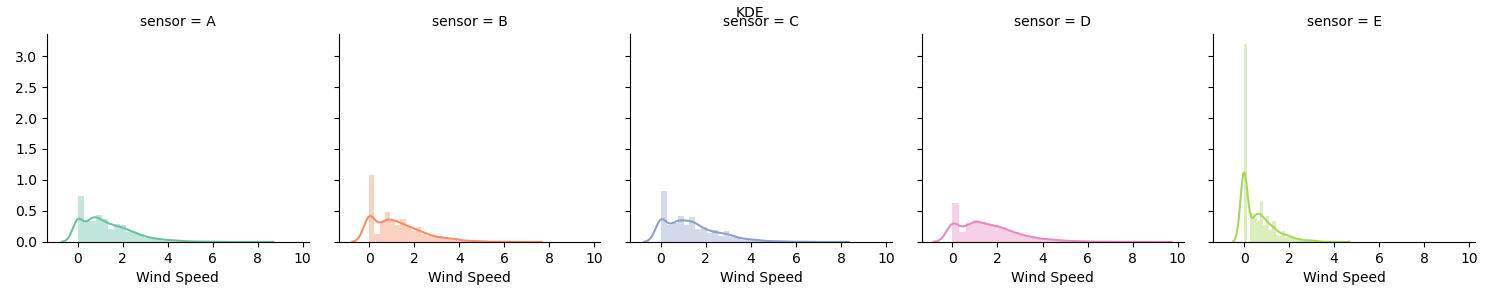
\includegraphics[width=17cm]{images/a2_3.png}
\centering
\caption{Wind speed PDF and KDE for sensor A-E plotted separately}
\end{figure}
In Figure 8, when only the KDE are plotted on a single graph, a significant difference in E is visible, indicating that there is some difference in the location of the sensor E which is leading to a different observation. 
\begin{figure}[H]
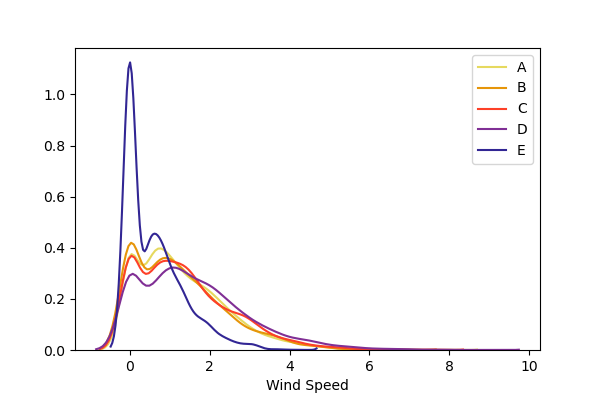
\includegraphics[width=17cm]{images/a2_4.png}
\centering
\caption{KDE plots of wind speed variable for sensors A-E aggregated}
\end{figure}

\newpage
\section{A3}
Figure 9 below shows the scatter plots of the pairwise correlations of variables Temperature, Wet Bulb Globe Temperature (WBGT) and Crosswind Speed between sensors A - E using Pearson's and Spearmann's rank coefficient. It is interesting to note that in both the correlation indices, both Temperature and WBGT have ranks of above 0.95 which is indicative of very strong correlations while for the variable crosswind speed, the correlations are all below 0.64 indicating a poor correlation. Even in these correlation plots, when comparing the coefficients of those correlations which had one component from sensor E, we see that all such coefficients happen to have lower correlation values in both Pearson's and Spearmann's correlation.
\begin{figure}[H]
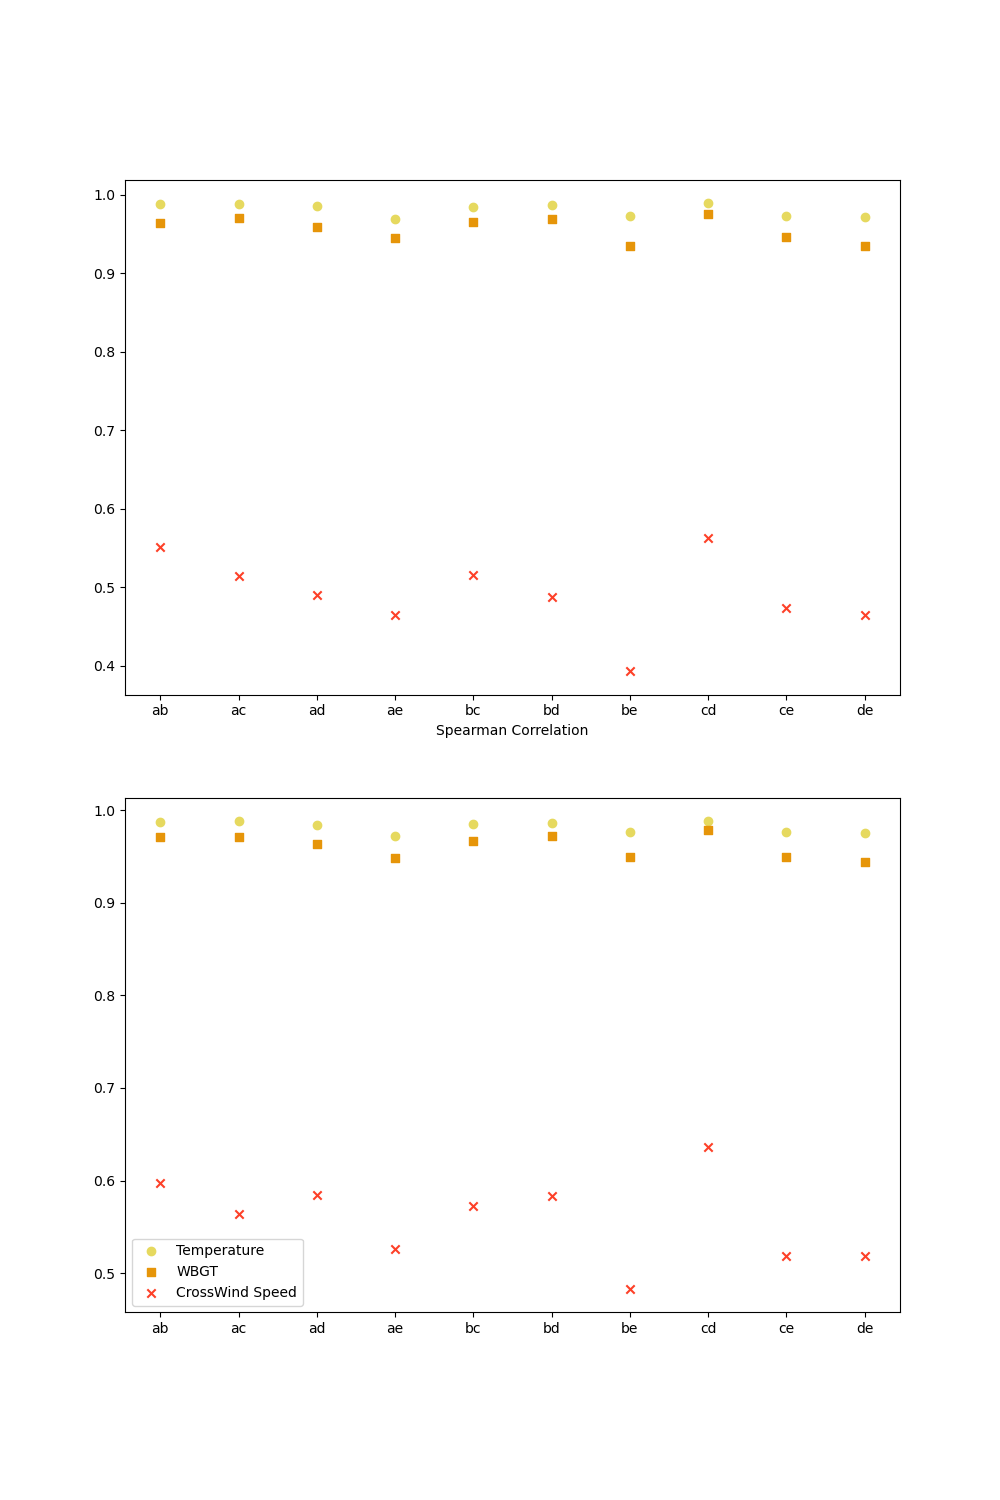
\includegraphics[width=12cm]{images/a3.png}
\centering
\caption{Scatterplot of Pearson and Spearman correlation coeefficients }
\end{figure}
Tables 2,3,4,5,6,7 show the correlation matices formed for the three variables in Pearson's and Spearmann's correlation methods.

%% tables spear cs
{
\small
\begin{table}[htbp]
  \centering
  \caption{Pairwise Spearmann's correlation of crosswind speed   }
  \resizebox{\textwidth}{!}{%
    \begin{tabular}{llllll}
                               & \textbf{Crosswind\_SpeedA} & \textbf{Crosswind\_SpeedB} & \textbf{Crosswind\_SpeedC} & \textbf{Crosswind\_SpeedD} & \textbf{Crosswind\_SpeedE} \\
    \textbf{Crosswind\_SpeedA} & 1.0                        & 0.5972402814921272         & 0.5637671399915773         & 0.5844814542499214         & 0.5261893084867895         \\
    \textbf{Crosswind\_SpeedB} & 0.5972402814921272         & 1.0                        & 0.5730301199997236         & 0.5836984945328472         & 0.4827979303236816         \\
    \textbf{Crosswind\_SpeedC} & 0.5637671399915773         & 0.5730301199997236         & 1.0                        & 0.6359061682587346         & 0.5189229541066187         \\
    \textbf{Crosswind\_SpeedD} & 0.5844814542499214         & 0.5836984945328472         & 0.6359061682587346         & 1.0                        & 0.5188518184856887         \\
    \textbf{Crosswind\_SpeedE} & 0.5261893084867895         & 0.4827979303236816         & 0.5189229541066187         & 0.5188518184856887         & 1.0                       
    \end{tabular}
    }
\end{table}
}

%%spear temp
{
\small
\begin{table}[htbp]
  \centering
  \caption{Pairwise Spearmann's correlation of Temperature}
  \resizebox{\textwidth}{!}{%
    \begin{tabular}{llllll}
                   & \textbf{TempA}     & \textbf{TempB}     & \textbf{TempC}     & \textbf{TempD}     & \textbf{TempE}     \\
    \textbf{TempA} & 1.0                & 0.9873816048765109 & 0.9880913733962015 & 0.9843597065082935 & 0.971679562373189  \\
    \textbf{TempB} & 0.9873816048765109 & 1.0                & 0.9852451592225194 & 0.9857684913050065 & 0.9767727006658334 \\
    \textbf{TempC} & 0.9880913733962015 & 0.9852451592225194 & 1.0                & 0.9881855891390962 & 0.9769209774377852 \\
    \textbf{TempD} & 0.9843597065082935 & 0.9857684913050065 & 0.9881855891390962 & 1.0                & 0.9753775047693785 \\
    \textbf{TempE} & 0.971679562373189  & 0.9767727006658334 & 0.9769209774377852 & 0.9753775047693785 & 1.0               
    \end{tabular}
    }
\end{table}
}
%%spear wbgt
{
\small
\begin{table}[htbp]
  \centering
  \caption{Pairwise Spearmann's correlation of  Wet Bulb Globe Temperature}
  \resizebox{\textwidth}{!}{%
    \begin{tabular}{llllll}
                   & \textbf{TempA}     & \textbf{TempB}     & \textbf{TempC}     & \textbf{TempD}     & \textbf{TempE}     \\
    \textbf{TempA} & 1.0                & 0.9873816048765109 & 0.9880913733962015 & 0.9843597065082935 & 0.971679562373189  \\
    \textbf{TempB} & 0.9873816048765109 & 1.0                & 0.9852451592225194 & 0.9857684913050065 & 0.9767727006658334 \\
    \textbf{TempC} & 0.9880913733962015 & 0.9852451592225194 & 1.0                & 0.9881855891390962 & 0.9769209774377852 \\
    \textbf{TempD} & 0.9843597065082935 & 0.9857684913050065 & 0.9881855891390962 & 1.0                & 0.9753775047693785 \\
    \textbf{TempE} & 0.971679562373189  & 0.9767727006658334 & 0.9769209774377852 & 0.9753775047693785 & 1.0               
    \end{tabular}
    }
\end{table}
}

%% pear cs
{
\small
\begin{table}[htbp]
  \centering
  \caption{Pairwise Pearson's correlation of Crosswind Speed }
  \resizebox{\textwidth}{!}{%
    \begin{tabular}{llllll}
                               & \textbf{Crosswind\_SpeedA} & \textbf{Crosswind\_SpeedB} & \textbf{Crosswind\_SpeedC} & \textbf{Crosswind\_SpeedD} & \textbf{Crosswind\_SpeedE} \\
    \textbf{Crosswind\_SpeedA} & 1.0                        & 0.5506880993864768         & 0.513967419205316          & 0.48979712009170695        & 0.4650585560284869         \\
    \textbf{Crosswind\_SpeedB} & 0.5506880993864768         & 1.0                        & 0.5160200947228815         & 0.48793745446153475        & 0.39266766187584295        \\
    \textbf{Crosswind\_SpeedC} & 0.513967419205316          & 0.5160200947228815         & 1.0                        & 0.5628881993613124         & 0.47304173448920345        \\
    \textbf{Crosswind\_SpeedD} & 0.48979712009170695        & 0.48793745446153475        & 0.5628881993613124         & 1.0                        & 0.46505234581136934        \\
    \textbf{Crosswind\_SpeedE} & 0.4650585560284869         & 0.39266766187584295        & 0.47304173448920345        & 0.46505234581136934        & 1.0                       
    \end{tabular}
    }
\end{table}
}

%%pear temp
{
\small
\begin{table}[htbp]
  \centering
  \caption{Pairwise Pearson's correlation of Temperature  }
  \resizebox{\textwidth}{!}{%
    \begin{tabular}{llllll}
                   & \textbf{TempA}     & \textbf{TempB}     & \textbf{TempC}     & \textbf{TempD}     & \textbf{TempE}     \\
    \textbf{TempA} & 1.0                & 0.9880982473187315 & 0.9886050426862583 & 0.985609473422632  & 0.969209007704399  \\
    \textbf{TempB} & 0.9880982473187315 & 1.0                & 0.9844805788828975 & 0.9862609463581227 & 0.9720922181749667 \\
    \textbf{TempC} & 0.9886050426862583 & 0.9844805788828975 & 1.0                & 0.9887428724207226 & 0.9720959224000858 \\
    \textbf{TempD} & 0.985609473422632  & 0.9862609463581227 & 0.9887428724207226 & 1.0                & 0.9713709593108307 \\
    \textbf{TempE} & 0.969209007704399  & 0.9720922181749667 & 0.9720959224000858 & 0.9713709593108307 & 1.0               
    \end{tabular}
    }
\end{table}
}

%%pear wbgt
{
\small
\begin{table}[htbp]
  \centering
  \caption{Pairwise Pearson's correlation of  Wet Bulb Globe Temperature}
  \resizebox{\textwidth}{!}{%
    \begin{tabular}{llllll}
                   & \textbf{WBGTA}     & \textbf{WBGTB}     & \textbf{WBGTC}     & \textbf{WBGTD}     & \textbf{WBGTE}     \\
    \textbf{WBGTA} & 1.0                & 0.9639274628697408 & 0.9706815061184246 & 0.9584355725847846 & 0.9443183165489981 \\
    \textbf{WBGTB} & 0.9639274628697408 & 1.0                & 0.9653368159749821 & 0.9691731015364442 & 0.9349541697294321 \\
    \textbf{WBGTC} & 0.9706815061184246 & 0.9653368159749821 & 1.0                & 0.9746813736059209 & 0.9460866144542396 \\
    \textbf{WBGTD} & 0.9584355725847846 & 0.9691731015364442 & 0.9746813736059209 & 1.0                & 0.9345082456136841 \\
    \textbf{WBGTE} & 0.9443183165489981 & 0.9349541697294321 & 0.9460866144542396 & 0.9345082456136841 & 1.0               
    \end{tabular}
    }
\end{table}
}

Drawing from all the conclusions discussed in the sections so far, the sensor E has shown many differences in the mean variance and standard deviation of the wind speed, wind direction and crosswind speeds while even in the distribution plotted using the PDF, PMF, boxplots of temperature wind speed and direction, similar conclusions have been drawn about sensor E, showing a behavior indicative of different environment in which its measurement has been taken. From the satellite image of the possible sensor locations as in Figure 10., it can be concluded that owing to the different environment at the top right location in the figure, should be the location of sensor E. The obtrusion to the flow of wind and availability of buildings around that spot explains the varied wind speed and direction obtained from sensor E. The longer tail of the CDF of sensor E in Figure 6 also explains this skew owing to urban heat island effect being created from the buildings around the sensor which trap heat.
Nothing much can be ascertained about the locations of the remaining sensors since they observe similar characteristics.


\begin{figure}[H]
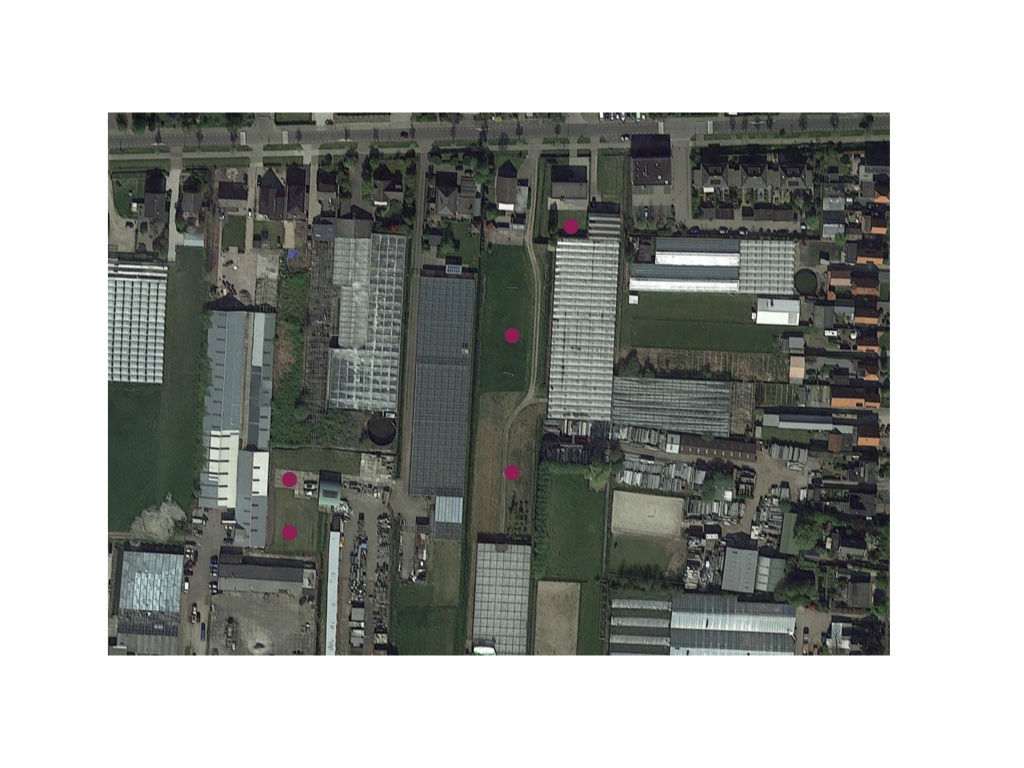
\includegraphics[width=19cm]{images/SensorsSketch.png}
\centering
\caption{ Satellite image with possible location of sensors}
\end{figure}


\newpage
\section{A4}
The CDF plots of wind speed and temperature values for all sensors in Figure 11., shows the following:
\begin{itemize}
  \item Wind Speed: The sensor E shows high percentage wind speeds in the category of 0 m/s meaning no wind and the maximum obtained is about 4-5m/s while in case of other sensors the maximum goes in the range of 7-8 m/s and 8.5 for sensor D. Thus strengthening our choice of location for sensor E in section A3.
  \item Temperature: Sensor E shows a larger tail in the temperature CDF indicating higher temperature owing to presence of buildings.
\end{itemize}

\begin{figure}[H]
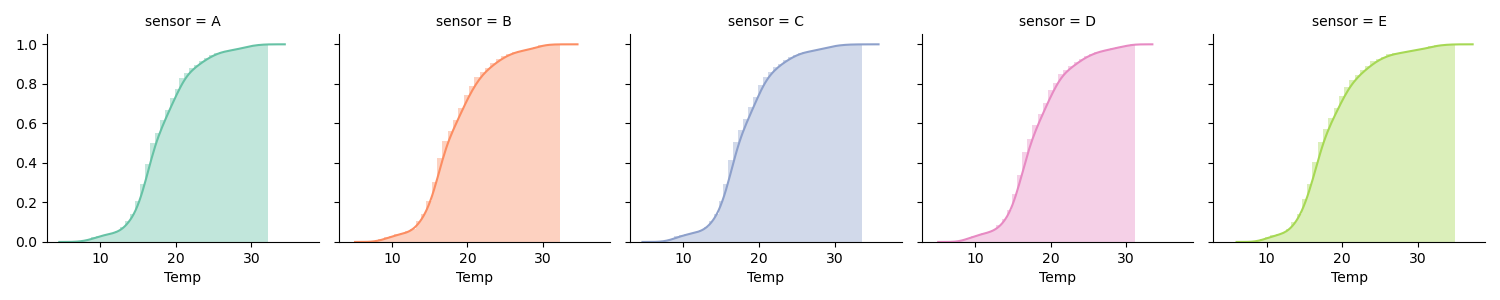
\includegraphics[width=17cm]{images/a4_1.png}
\centering
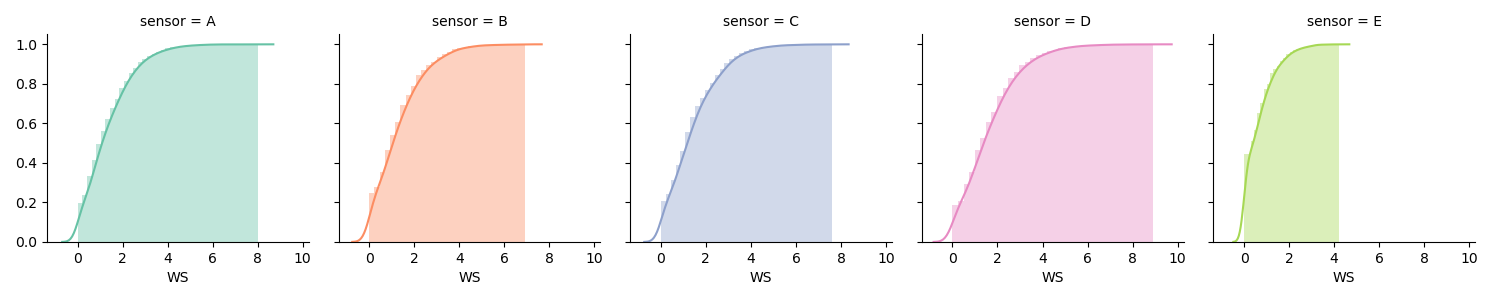
\includegraphics[width=17cm]{images/a4_2.png}
\centering
\caption{ CDF plots of Temperature (top) and Wind speed (bottom) for each sensor}
\end{figure}

Table 8 indicates the confidence intervals obtained for Temperature and wind speed for sensors A-E for an \alpha{} value of 0.05 or 95\% confidence

{
\small
\begin{table}[htbp]
  \centering
  \caption{Confidence intervals of Temperature and wind speed variables of all sensors}
  \resizebox{\textwidth}{!}{%
    \begin{tabular}{llllll}
    \hline
                         & \multicolumn{1}{c}{\textbf{A}} & \multicolumn{1}{c}{\textbf{B}} & \multicolumn{1}{c}{\textbf{C}} & \multicolumn{1}{c}{\textbf{D}} & \multicolumn{1}{c}{\textbf{E}} \\ \hline
    \textbf{Temperature} & 0.15696225989519724            & 0.16070121021566336            & 0.1582103857966651             & 0.1582155582881216             & 0.1720054479116186             \\
    \textbf{Wind Speed}  & 0.04407990769723572            & 0.04495805948624314            & 0.04715942886670751            & 0.05200110920681511            & 0.02818251904758019            \\ \hline
    \end{tabular}
    }
\end{table}
}

In order to test the hypothesis: the time series for Temperature and Wind Speed are the same for sensors, we should take a null hypothesis such that:
\begin{itemize}
  \item N\textsubscript{0} : Time series are the same
  \item N\textsubscript{0} : Time series are diffeent
\end{itemize}
Now for the null hypothesis to be rejected, we need to look at the p-values obtained for the students test run on the two sensors, which can be seen in Table 9 below.
\begin{itemize}
  \item If p-value is < alpha => N\textsubscript{0} is rejected
  \item If p-value is > alpha => N\textsubscript{0} is not rejected
\end{itemize}
From the Table 9., it is evident that the time series of Temperature of sensors ED is not same while the time series of wind speed of sensors ED, DC and CB are not the same.

{
\small
\begin{table}[htbp]
  \centering
  \caption{p-values for temperature and wind speed variables for all sensors}
  \begin{tabular}{lll}
                 & \textbf{Temp} & \textbf{Wind Speed}           \\
    \textbf{E-D} & 0.0027        & 3.37*10\textsuperscript{-212} \\
    \textbf{D-C} & 0.4658        & 4.61*10\textsuperscript{-09}                      \\
    \textbf{C-B} & 0.1855        & 0.0001                        \\
    \textbf{B-A} & 0.4005        & 0.1335                       
    \end{tabular}
    
\end{table}
}


\newpage
\bibliographystyle{apacite}
\bibliography{ref.bib}

\end{document}